\section{User Inputs}
In an era before Microsoft harnessed all inputs under DirectInput API with Windows 95, developers had to write drivers for each input type they wanted to support. This involved talking directly to the hardware in the vendor's protocol on a physical port. The keyboard is plugged into a PS/2, the mouse to a serial port (DE9), and the joystick to a game port (DA-15) on the SoundBlaster.





\subsection{Keyboard}

As the keyboard is the standard and oldest input medium, it is fairly easy to access. When a key is pressed, the interrupt is routed to an ISR in the Vector Interrupt Table. The engine installs its own ISR there.


\par
\begin{minipage}{\textwidth}
\lstinputlisting[language=C]{code/keyboard.c}
\end{minipage}

The state of the keyboard is maintained in a global array \cw{Keyboard}, available for the entire engine to lookup.\\
\par

\begin{minipage}{\textwidth}
\lstinputlisting[language=C]{code/keyboard_array.c}
\end{minipage}



\subsection{Mouse}
A driver has to be loaded at startup for the mouse to be accessible. Beginning with DOS 5, operating systems had a default driver. It had to be added to \cw{config.sys} so it would reside in RAM.\\
\par 
\begin{minipage}{\textwidth}
\lstinputlisting[language=C]{code/mouse.sys.c}
\end{minipage}
The driver takes almost 5KiB of RAM. With the driver loaded all interactions happen with software interrupt \cw{0x33}. The interface works with request issued in register AX and response issued in registers CX, BX and DX. With Borland compiler syntactic sugar it is easy to write with almost no boilerplate (notice direct access to registers thanks to \_AX and co special keywords.)\\
\par
\begin{minipage}{\textwidth}
\lstinputlisting[language=C]{code/mouse_request.c}
\end{minipage}
\par
\begin{minipage}{\textwidth}
\begin{figure}[H]
\centering
\begin{tabularx}{\textwidth}{ >{\hsize=.5\hsize}X  >{\hsize=.5\hsize}X  X }
  \toprule
  \textbf{Request} & \textbf{Type} & \textbf{Response} \\ \bottomrule
AX=0 & Get Status & AX = FFFFh : available. AX Value = 0 : not available\\
AX=1 & Show Pointer & \\
AX=2 & Hide Pointer & \\
AX=3 & Mouse Position & CX = X Coordinate, DX = Y Coordinate\\
AX=3 & Mouse Buttons & BX = 1 Left Pressed, BX = 2 Right Pressed, BX = 3 Center Button Pressed\\
AX=7 & Set Horizontal Limit & CX=MaxX1 DX=MaxX2\\
AX=8 & Set Vertical Limit & CX=MaxY1 DX=MaxY2\\
\bottomrule
\end{tabularx}
\caption{Mouse request/response.}
\end{figure}
\end{minipage}
\par









\subsection{Joystick}
All interactions with the joystick happen over I/O port \cw{0x201}. Two joysticks can be chained together and the state of both of them fits in a byte.\\ 
\par
\begin{minipage}{\textwidth}
\lstinputlisting[language=C]{code/joystick.c}
\end{minipage}
\par



\begin{figure}[H]
\centering
\begin{tabularx}{\textwidth}{ >{\hsize=.5\hsize}X X  }
  \toprule
  \textbf{Bit Number} & \textbf{Meaning} \\ \bottomrule
0 & Joystick A, X Axis \\
1 & Joystick A, Y Axis \\
2 & Joystick B, X Axis \\ 
3 & Joystick B, Y Axis \\
4 & Joystick A, Button 1 \\
5 & Joystick A, Button 2 \\
6 & Joystick B, Button 1 \\
7 & Joystick B, Button 2 \\
\bottomrule
\end{tabularx}
\caption{Joystick sampling bit and their meaning.}
\end{figure}
\par
The API looks clean at first with each button associated to a bit indicating if it is pressed or not. But if you take a closer look you will notice there is only one bit of information per axis which is not enough to encode the position of a stick. This bit is actually a flag allowing to convert an analog input into a digital value. To understand better, let's dive into details. On the joystick side, each axis is connected to a 100k$\Omega$ potentiometer. An applied 5V voltage generates a variable current based on the stick position (remember Ohm law where $I = \frac{V}{R}$).\\ 
\par
\begin{figure}[H]
\centering
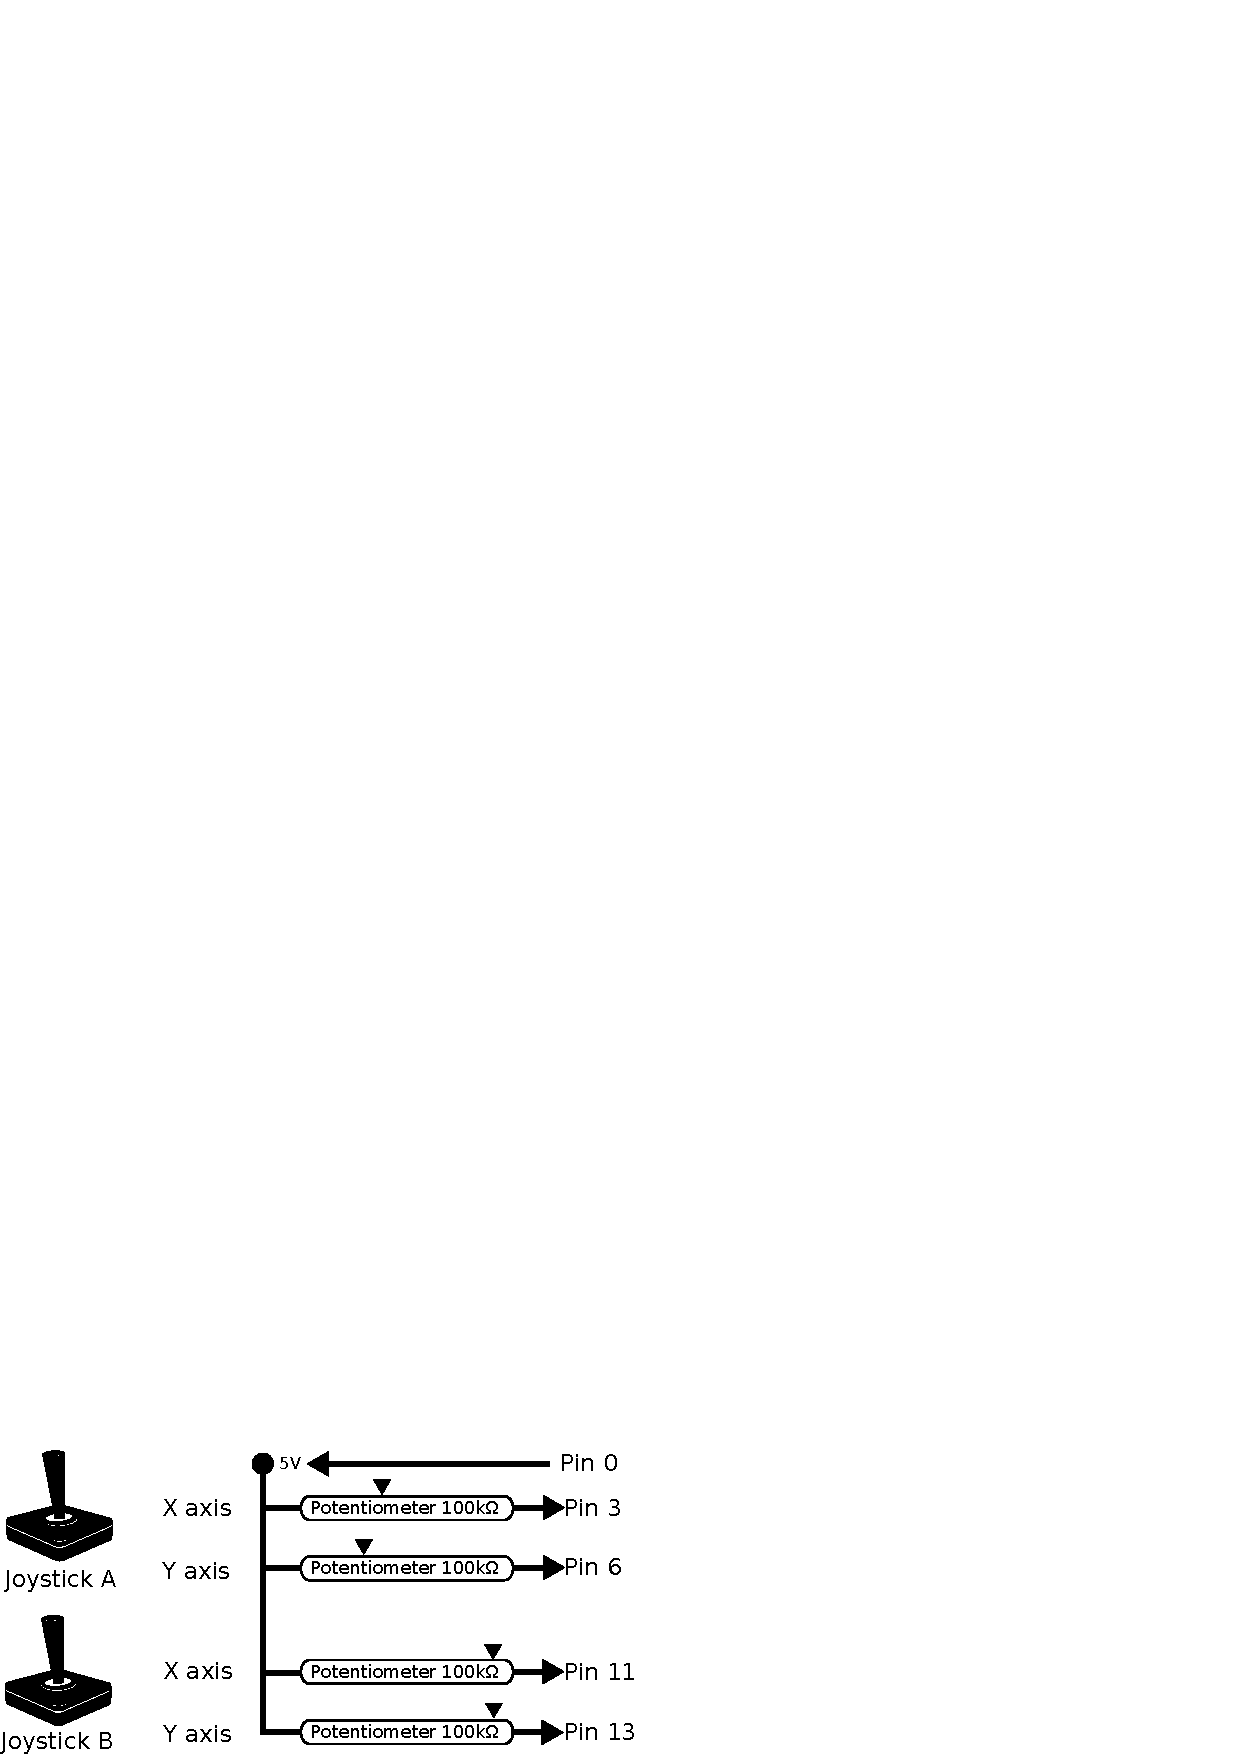
\includegraphics[width=\textwidth]{imgs/drawings/joystick_potentiometers.pdf}
\end{figure}
\par
On the game controller side the pin carrying the current are connected to monostable multivibrators. Which is a complicated name for a capacitor able to output 1 when it is charged and 0 when it is charging. The idea is to infer the position of the stick by measuring how long the vibrator takes to charge (a strong current will charge the capacitor faster than a weak current).\\
\par
\par
\begin{figure}[H]
\centering
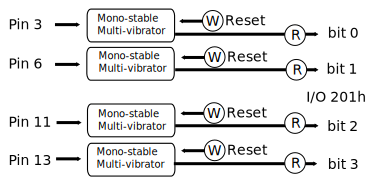
\includegraphics[width=\textwidth]{imgs/drawings/joystick_gamecontroller.pdf}
\end{figure}
\par
On the CPU side the idea is to empty the capacitor and measure how long it took to re-charge. It is done in three steps:

\begin{itemize}
 \item Write \circled{W} any value to I/O port \cw{201h}. This will discharge the vibrators.
 \item Initialize a counter to zero and read \circled{R} from \cw{201h}. At first all bit 0-4 will be equal to zero.
 \item Loop forever (or when counter == 0xFFFF as safety measure). Save at which loop count a bit flipped to 1.
\end{itemize}
\par
On a 286 CPU the values for each axis can range from 7 to 900 depending on the stick/capacitor position. On a 386 CPU which will run loops faster these value would be smaller. Hence these absolute value can only be translated to a stick position if they are compared to the min and max value.\\
\par Which explains why joysticks have to be calibrated. For the flight simulators of the 90s where accurate position was needed, the player would be asked to put the joystick in upper-left position (to set the potentiometers on both axis to minimum resistance) and press a button to read the "loop count". Repeat the operation at lower right position and you know what are the min and max "loop count" for this joystick/CPU combination.\\
\par
\begin{figure}[H]
\centering
\fullimage{joystick_calibration.png}
\caption{Strike Commander startup screen makes you calibrate your joystick.}
\end{figure}
\par
There is no calibration process in Wolfenstein 3D because when the engine starts up it samples the loop count and assume the joystick was in neutral position. When the game runs and joystick position is needed, the engine samples loop count and compare the count to what was measured with neutral. It is not enough to calculate the exact stick position on each axis but it is enough to determine if it was up/down and left/right using >, == (with epsilon) and < comparison operations.